\section{Date: 2026-08-02}
\noindent \textbf{Series ID: MORTMRGN1W} 

\noindent This series is titled Margin for 1-Year Adjustable Rate Mortgage in the West Freddie Mac Region (DISCONTINUED) and has a frequency of Weekly, Ending Thursday. The units are Percent and the seasonal adjustment is Not Seasonally Adjusted.The observation start date is 1988-02-19 and the observation end date is 2015-12-31.The popularity of this series is 1. \\ 

\noindent \textbf{Series ID: ISRRECD} 

\noindent This series is titled OECD based Recession Indicators for Israel from the Period following the Peak through the Trough (DISCONTINUED) and has a frequency of Daily, 7-Day. The units are +1 or 0 and the seasonal adjustment is Not Seasonally Adjusted.The observation start date is 1995-02-01 and the observation end date is 2022-09-30.The popularity of this series is 1. \\ 

\subsection{Raw Regression}
\noindent Regresses the two series against each other directly. A significant result here can come just as easily from both series sharing a long-run trend as from any real relationship.

\begin{center}
\begin{tabular}{lclc}
\toprule
\textbf{Dep. Variable:}          & value\_fred\_ISRRECD & \textbf{  R-squared:         } &     0.000   \\
\textbf{Model:}                  &         OLS          & \textbf{  Adj. R-squared:    } &    -0.001   \\
\textbf{Method:}                 &    Least Squares     & \textbf{  F-statistic:       } &    0.2199   \\
\textbf{Date:}                   &   Sun, 02 Aug 2026   & \textbf{  Prob (F-statistic):} &    0.639    \\
\textbf{Time:}                   &       12:49:41       & \textbf{  Log-Likelihood:    } &   -776.50   \\
\textbf{No. Observations:}       &          1091        & \textbf{  AIC:               } &     1557.   \\
\textbf{Df Residuals:}           &          1089        & \textbf{  BIC:               } &     1567.   \\
\textbf{Df Model:}               &             1        & \textbf{                     } &             \\
\textbf{Covariance Type:}        &      nonrobust       & \textbf{                     } &             \\
\bottomrule
\end{tabular}
\begin{tabular}{lcccccc}
                                 & \textbf{coef} & \textbf{std err} & \textbf{t} & \textbf{P$> |$t$|$} & \textbf{[0.025} & \textbf{0.975]}  \\
\midrule
\textbf{const}                   &       0.6995  &        0.602     &     1.161  &         0.246        &       -0.483    &        1.882     \\
\textbf{value\_fred\_MORTMRGN1W} &      -0.1029  &        0.219     &    -0.469  &         0.639        &       -0.533    &        0.328     \\
\bottomrule
\end{tabular}
\begin{tabular}{lclc}
\textbf{Omnibus:}       & 4409.818 & \textbf{  Durbin-Watson:     } &    0.038  \\
\textbf{Prob(Omnibus):} &   0.000  & \textbf{  Jarque-Bera (JB):  } &  182.321  \\
\textbf{Skew:}          &   0.337  & \textbf{  Prob(JB):          } & 2.57e-40  \\
\textbf{Kurtosis:}      &   1.114  & \textbf{  Cond. No.          } &     125.  \\
\bottomrule
\end{tabular}
%\caption{OLS Regression Results}
\end{center}

Notes: \newline
 [1] Standard Errors assume that the covariance matrix of the errors is correctly specified.

\begin{figure}
\centering
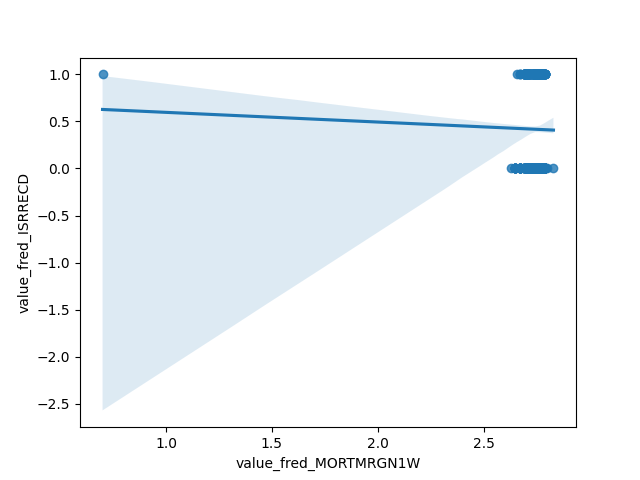
\includegraphics[scale = 0.9]{plots/plot_2026-08-02.png}
\caption{Raw Regression Plot for 2026-08-02}
\end{figure}
\newpage
\subsection{Detrended Regression}
\noindent Regresses the residuals of each series after removing its own linear time trend, so a shared trend can no longer drive the result on its own. A relationship that stays significant here is better evidence of a genuine link between the two series.

\begin{center}
\begin{tabular}{lclc}
\toprule
\textbf{Dep. Variable:}                     & value\_fred\_ISRRECD\_detrended & \textbf{  R-squared:         } &     0.001   \\
\textbf{Model:}                             &               OLS               & \textbf{  Adj. R-squared:    } &    -0.000   \\
\textbf{Method:}                            &          Least Squares          & \textbf{  F-statistic:       } &    0.9398   \\
\textbf{Date:}                              &         Sun, 02 Aug 2026        & \textbf{  Prob (F-statistic):} &    0.333    \\
\textbf{Time:}                              &             12:49:41            & \textbf{  Log-Likelihood:    } &   -774.85   \\
\textbf{No. Observations:}                  &                1091             & \textbf{  AIC:               } &     1554.   \\
\textbf{Df Residuals:}                      &                1089             & \textbf{  BIC:               } &     1564.   \\
\textbf{Df Model:}                          &                   1             & \textbf{                     } &             \\
\textbf{Covariance Type:}                   &            nonrobust            & \textbf{                     } &             \\
\bottomrule
\end{tabular}
\begin{tabular}{lcccccc}
                                            & \textbf{coef} & \textbf{std err} & \textbf{t} & \textbf{P$> |$t$|$} & \textbf{[0.025} & \textbf{0.975]}  \\
\midrule
\textbf{const}                              &   -1.427e-13  &        0.015     & -9.57e-12  &         1.000        &       -0.029    &        0.029     \\
\textbf{value\_fred\_MORTMRGN1W\_detrended} &      -0.2216  &        0.229     &    -0.969  &         0.333        &       -0.670    &        0.227     \\
\bottomrule
\end{tabular}
\begin{tabular}{lclc}
\textbf{Omnibus:}       & 4445.590 & \textbf{  Durbin-Watson:     } &    0.039  \\
\textbf{Prob(Omnibus):} &   0.000  & \textbf{  Jarque-Bera (JB):  } &  180.416  \\
\textbf{Skew:}          &   0.337  & \textbf{  Prob(JB):          } & 6.66e-40  \\
\textbf{Kurtosis:}      &   1.125  & \textbf{  Cond. No.          } &     15.3  \\
\bottomrule
\end{tabular}
%\caption{OLS Regression Results}
\end{center}

Notes: \newline
 [1] Standard Errors assume that the covariance matrix of the errors is correctly specified.

\begin{figure}
\centering
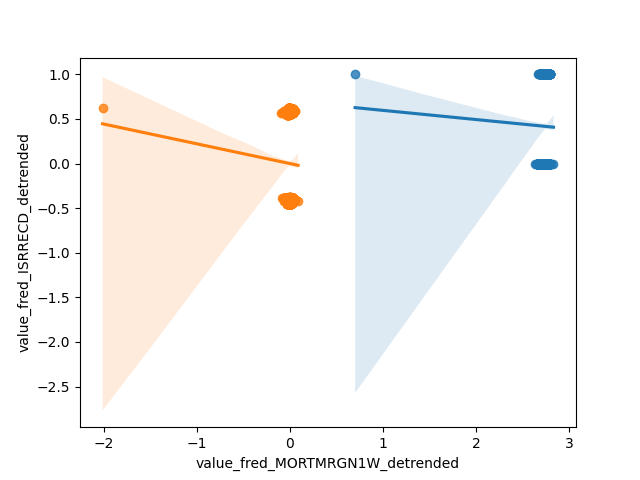
\includegraphics[scale = 0.9]{plots/plot_2026-08-02_detrended.png}
\caption{Detrended Regression Plot for 2026-08-02}
\end{figure}
\newpage
